\section{Case Study}
In this section, we demonstrate that with the metadata automatically normalized and expanded using the techniques in previous section, we are able to implement a few applications that are generalizable from one building to another building without modification. As a proof of cncept, we implment two applications: a) identify the uncomfortable rooms and b) detect rogues rooms. We also evaluate the metadata expansion technique in terms of the accuracy for both applications compared against the ground truth. 

\subsection{Experimental Setup}
We implement two applications and perform the analysis on two buildings from a campuses, and each building is installed with a different management system. Building A was built in mid-1990s using the system from Barrington ~\cite{}. Building B was recently built in 2005 using the Siements BACnet system~\cite{}. We collected temperature data as well as setpoint of the rooms in each building. And the data used from each building for analysis is from one week in June 2009 and January 2012 respectively.

\begin{figure*}[h!]
\centering
	\begin{subfigure}{0.48\textwidth}
                \centering
		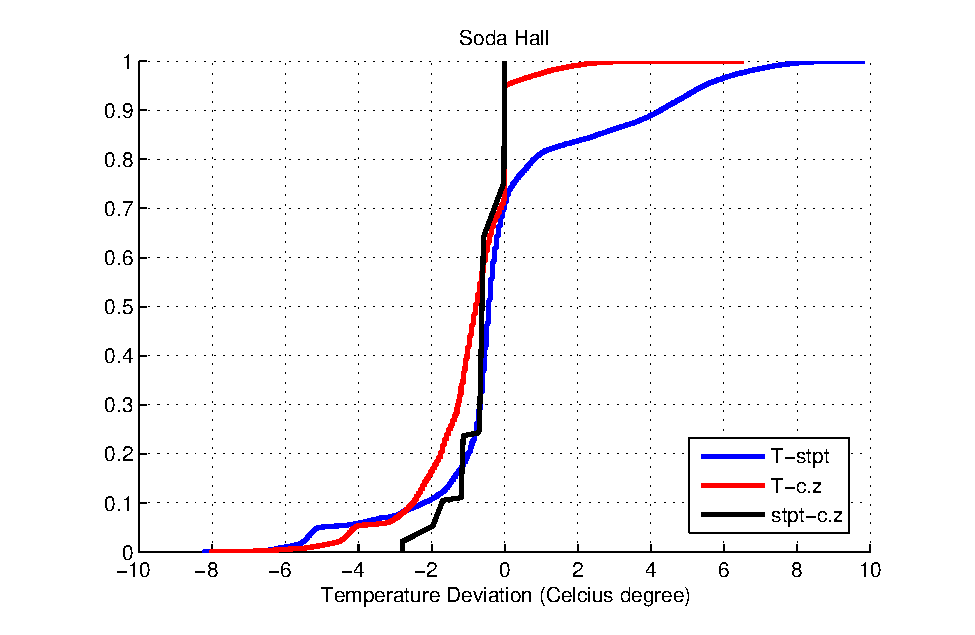
\includegraphics[width=\textwidth]{./figs/Soda_new.eps}
                \caption{Building A}
	\end{subfigure}
	\begin{subfigure}{0.48\textwidth}
                \centering
		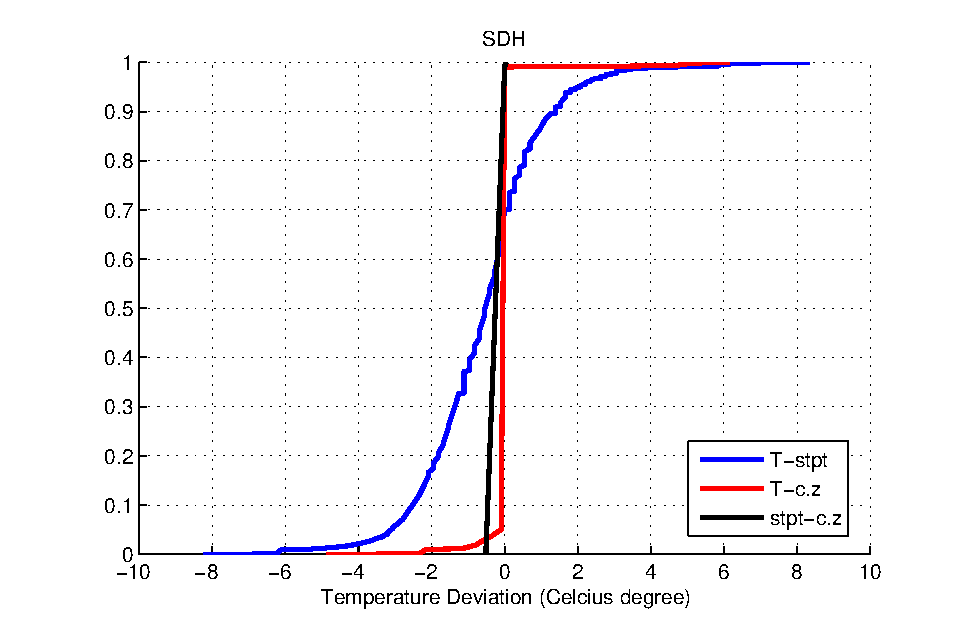
\includegraphics[width=\textwidth]{./figs/SDH_new.eps}
                \caption{Building B}
	\end{subfigure}
	% \begin{subfigure}{0.32\textwidth}
 %                \centering
	% 	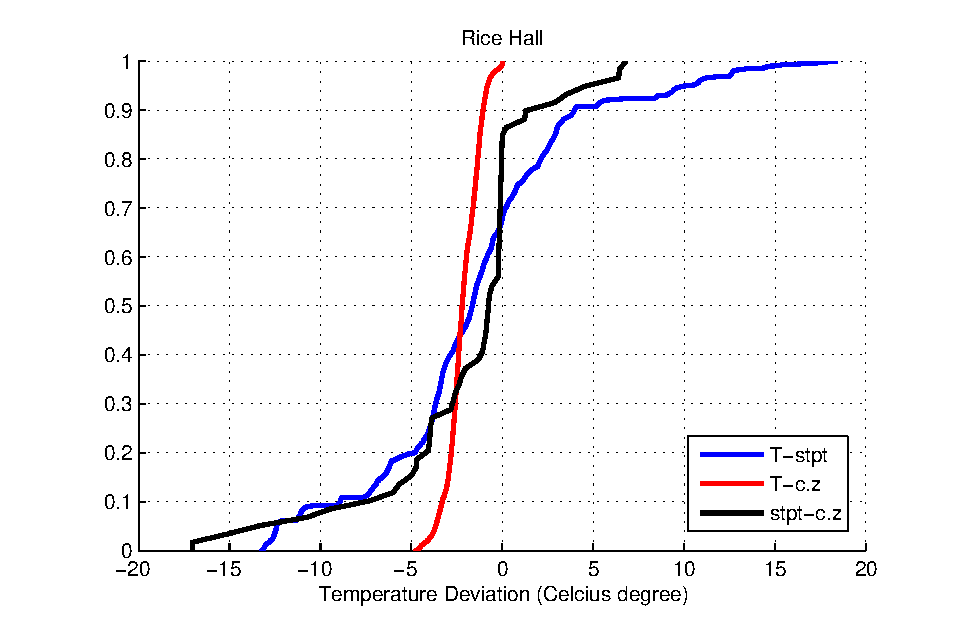
\includegraphics[width=\textwidth]{./figs/Rice_new.eps}
 %                \caption{Building C}
	% \end{subfigure}
\caption{For each building, we present the distribution of temperature deviation between: a) room temperature and the corresponding setpoint (solid), b) room temperature and the comfort range suggested by ASHRAE (dashed), c) room temperature setpoint and the ASHARE comfort suggestion (dotted).}
\label{fig:cdf_temp}
\end{figure*}

\begin{figure*}[h!]
\centering
	\begin{subfigure}{0.48\textwidth}
                \centering
		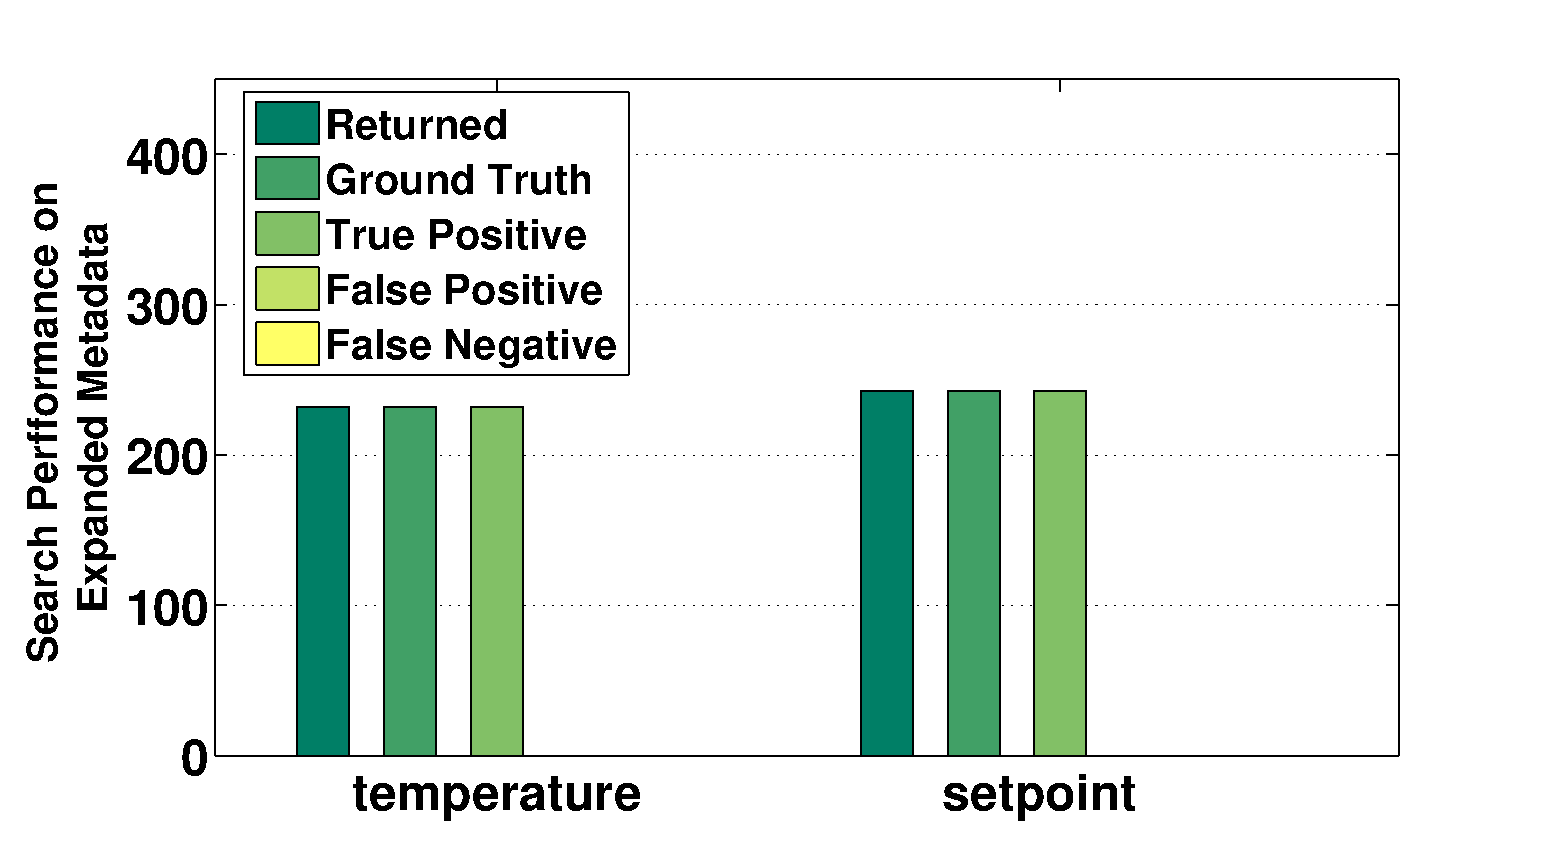
\includegraphics[width=\textwidth]{./figs/50-soda.eps}
                \caption{Building A}
	\end{subfigure}
	\begin{subfigure}{0.48\textwidth}
                \centering
		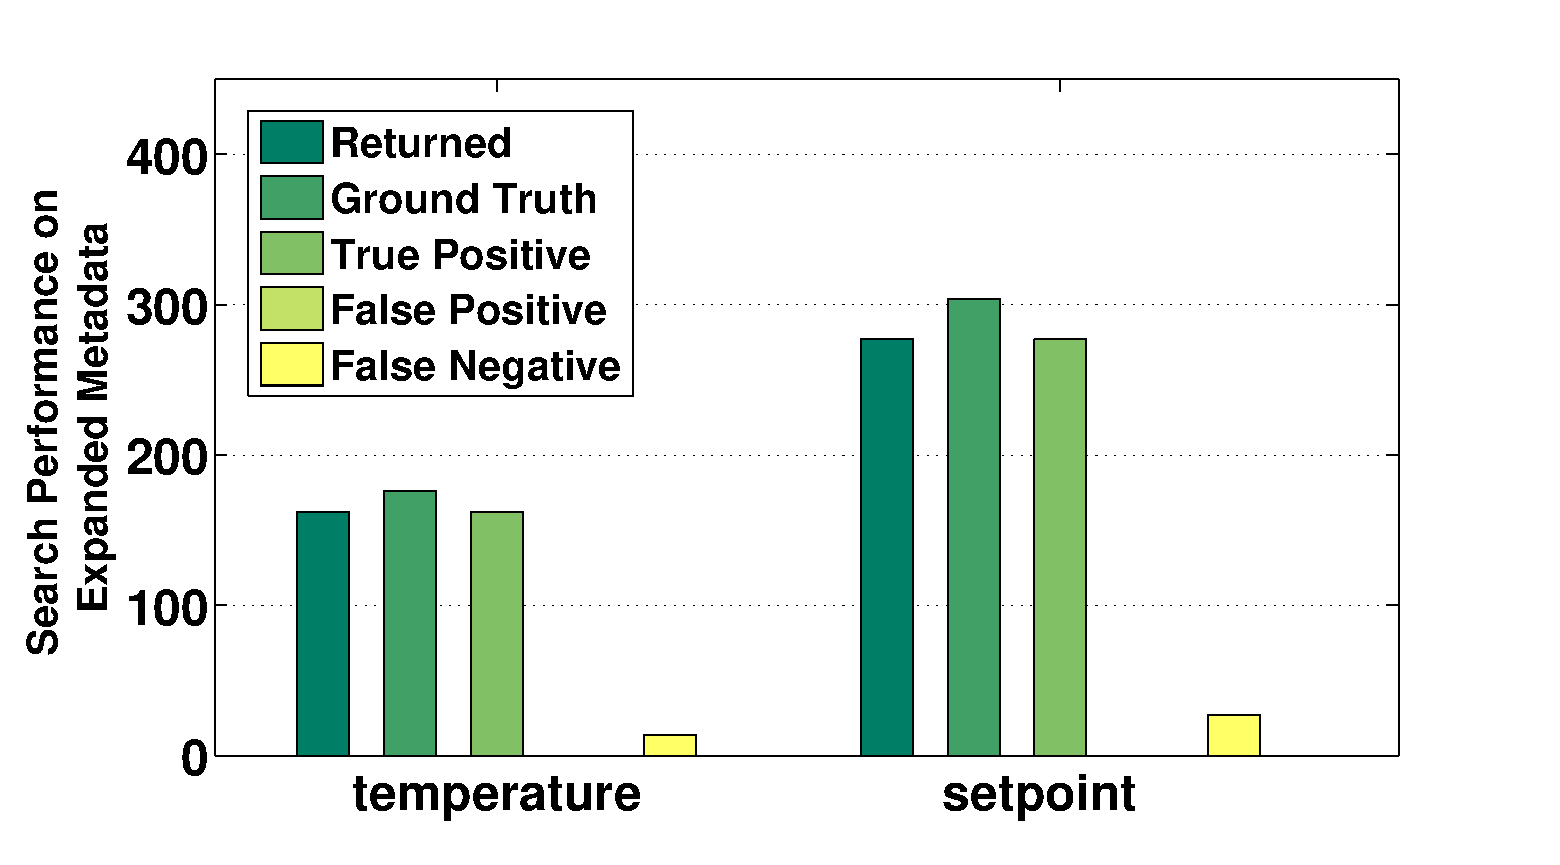
\includegraphics[width=\textwidth]{./figs/50-sdh.eps}
                \caption{Building B}
	\end{subfigure}
\caption{The error rates of searches over the expanded metadata using our techniques. We do two searches particularly: ``room temp'' and ``room temp setpoint''.}
\label{fig:cdf_temp}
\end{figure*}

\subsection{Uncomfortable Rooms}
It's not unusual to have rooms in a building stay extremely cold or hot thus making the occupants uncomfortable as well as incurring energy waste. The uncomfort are usually caused by improper setpoint settings or dysfunciton of the HVAC systems, and being able to identify these uncomfortable zones or rooms in the building is vital to occupant comfort as well as potential energy savings. With the metadata normalized using our techniques, we are able to search for the desired streams, e.g., the temperature and setpoint of a room,  and analyse the thermal performance across different buildings despite of the different naming schema of the sensor or ``points''.

To identify potential uncomfort in a building, for each room we are particularly interested in a) how much does the temperture deviate from the comfort range? b) how much does the temperature deviate from the setpoint? c) how much does the setpoint deviate from the comfort range? To answer these questions, we first search over the points in each building for distinct temperature stream of each room and the corresponding setpoint. And then we compare the temperature with setpoint as well as the suggested comfort range from ASHRAE~\cite{} to compute the temperature deviations in the aforementioned three different perspectives in the one-week period. We accumulate the results from all the rooms per building and generate the CDF as shown in Figure~\ref{}. Each graph illustrates how much the temperature of a building deviates from the comfort range, the setpoint and also, how much the setpoint by itself deviates from the comfort rage. On average, each buidling is uncomfortable to some degree and we rank the rooms in each building by how much they deviates from the comfort zone and the ranking is shown in Table~\ref{}. We also present the ground truth of temperature deviation distribution in Figure~\ref{fig:cdf_temp}, where we manually find temperature and setpoint streams for all the rooms to do the same analysis and generate the graphs. The ground truth analysis covers all the rooms in each building so all the potential uncomfortable rooms will be identified while the analysis using the name points expanded with our techniques would miss some of the uncomfortable rooms, since the expansion contains certain error rates.

\subsection{Rogue Rooms}
Heating and cooling contribute to the largest portion of energy consumption of a buidling, and often, HVAC system operates abnormally either because the system fails itself or the schedule of the buidling is problematic. And there are often some zones and rooms in a building that are constantly cold or hot than their neighbors and incur energy waste. We showed the temeprature deviations above, and we are particularly interested in the periods when a room deviates from the setpoint more than 3 Celsius degree, which is highly likely to indicate that the room is under either heating or coolong. Therefore, for each building, we zoom in to the interested portion and find the rooms whose percentage of time that falls into the interested area is extremely high, i.e., which room's temperature deviates from the setpoint more than 3 Celsius degree in most of the time, and the results are summarized in Table~\ref{}. Again, the grounf truth results are listed in Table~\ref{} as comparison.

\begin{table}[ht!]
%\footnotesize
 \begin{center}
	\begin{tabular}{|c|c|c|c|c|c|}
	\multicolumn{2}{c}{$Bldg A$}
	 & \multicolumn{2}{c}{$Bldg B$}
	  & \multicolumn{2}{c}{$Bldg C$} \\
	\cline{1-6} 
	 room\# & \% & room\# & \% & room\# & \%\\
	\cline{1-6}
	 330B & 1 & S3-6 & 1 & 501 & 1\\
	\cline{1-6}
	 340 & 1 & S2-1 & 1 & 502 & 1\\
	\cline{1-6}
	420A & 1 & S1-2 & 0.93 & 504 & 1\\
	\cline{1-6}
	420 & 1 & S7-16 & 0.67 & 557 & 1\\
	\cline{1-6}
	698 & 1 & S3-13 & 0.62 & 511A & 1\\
	\cline{1-6}
	442 & 0.996 & S4-15 & 0.62 & 532 & 1\\
	\cline{1-6}
	398 & 0.981 & S5-5 & 0.57 & 224 & 1\\
	\cline{1-6}
	336 & 0.96 & S4-1 & 0.54 & 506 & 1\\
	\cline{1-6}
	183 & 0.92 & S5-16 & 0.48 & 507 & 1\\
	\cline{1-6}
	498 & 0.91 & S5-7 & 0.47 & 511B & 1\\
	\cline{1-6}
	\end{tabular}
 \end{center}
 \caption{We present the ground truth for rooms in each building whose temperature deviates from the setpoint more than 3 Celsius degree. For each building, the first column is room number and the second column shows the percentage of the one-week time that the room deviates that much.}
 \label{tab:cluster}
\end{table}

\begin{figure*}[h!]
\centering
	\begin{subfigure}{0.48\textwidth}
                \centering
		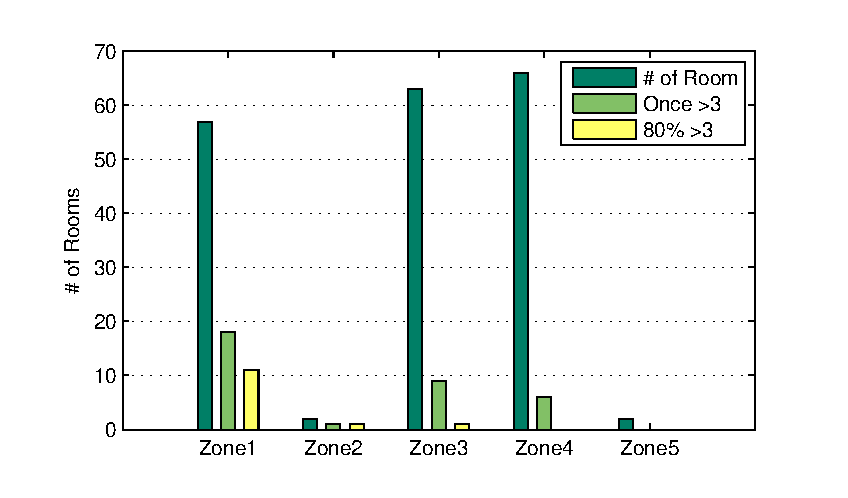
\includegraphics[width=\textwidth]{./figs/rogue_soda.eps}
                \caption{Building A}
	\end{subfigure}
	\begin{subfigure}{0.48\textwidth}
                \centering
		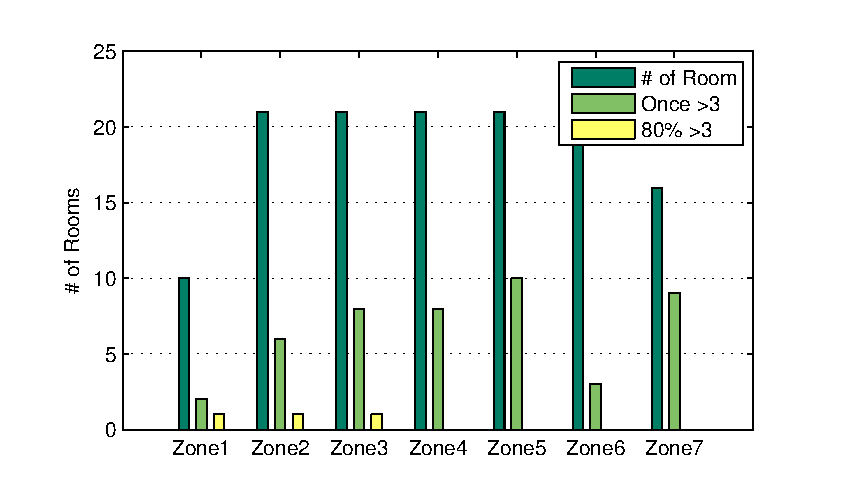
\includegraphics[width=\textwidth]{./figs/rogue_sdh.eps}
                \caption{Building B}
	\end{subfigure}
\caption{Dividing the rooms whose temperature once deviates from the setpoint more than 3 Celsius degree by HVAC zones: for each zone, we show the number of rooms in the zone, the number of zones once appears to be rogue, and the number of rooms that were rogues more than 80\% in the one-week period.} 
\label{fig:rogue}
\end{figure*}